
\documentclass[10pt]{exam}
\usepackage{graphicx}
\usepackage{listings}

\newcommand{\R}{\mathbb{R}}
\newcommand{\changes}[1]{{\color{red} #1}}
\usepackage{xcolor}
\usepackage[english]{babel}
\usepackage{amsmath,amssymb,amsthm,mathdots}
\usepackage{graphicx}
\usepackage[colorinlistoftodos]{todonotes}


\renewcommand{\thequestion}{\arabic{question} }
\renewcommand\questionlabel{\llap{\thequestion)}}


\usepackage{xcolor}
\definecolor{SolutionColor}{rgb}{0.1,0.3,1}

\unframedsolutions
\shadedsolutions
\definecolor{SolutionColor}{rgb}{0.9,0.9,1}
\renewcommand{\solutiontitle}{\textbf{Solution}$:\>$  }




%Mathcal and 
\newcommand{\mb}[1]{\mathbb{#1}}
\newcommand{\mc}[1]{\mathcal{#1}}

%Various possibilities for norms
\newcommand{\norm}[2]{\|#1\|_{#2}}
\newcommand{\normtwo}[1]{\|#1\|_{2}}
\newcommand{\normp}[1]{\|#1\|_{p}}

\newcommand{\rn}{\mathbb{R}^n}
\newcommand{\rnn}{\mathbb{R}^{n\times n}}
\newcommand{\rmn}{\mathbb{R}^{m\times n}}



%Boldface for vectors and tildes
\renewcommand{\vec}[1]{{#1}•}
\newcommand{\mat}[1]{{#1}•}

\newcommand{\vect}[1]{\widetilde{\boldsymbol{#1}}}
\newcommand{\matt}[1]{\widetilde{\boldsymbol{#1}}}

%Column and row equivalence
\newcommand{\roweq}{\stackrel{\text{row}}{\sim}}
\newcommand{\coleq}{\stackrel{\text{col}}{\sim}}

\newtheorem{definition}{Definition}
\newtheorem{example}{Example}
\newtheorem{fact}{Fact}
\newtheorem{remark}{Remark}


%Vector spaces
\newcommand{\rank}{\text{rank}\,}
\renewcommand{\dim}{\text{dim}\,}
\newcommand{\Span}[1]{\text{Span}\,\{#1\}}
\newcommand{\basis}[1]{\left\{ #1\right\}}


%Matrix environments
\newcommand{\bmat}[1]{\begin{bmatrix}#1\end{bmatrix}}
\newcommand{\pmat}[1]{\begin{pmatrix}#1\end{pmatrix}}
\newenvironment{amatrix}[1]{%
  \left(\begin{array}{@{}*{#1}{c}|c@{}}
}{%
  \end{array}\right)
}


%Trace and determinant
\newcommand{\diag}{\mathsf{diag}\,}
\newcommand{\range}{\mathsf{range}\,}
\newcommand{\trace}{\mathsf{trace}\,}


\usepackage{hyperref}
\title{MA 402: Project 3}
\author{Richard Watson, Mountain Chan, Cole Nash}
%\date{}
\begin{document}
\maketitle
\textbf{Instructions}: 

\begin{itemize}
\item Detailed instructions regarding submission are available on the class website\footnote{\url{https://github.ncsu.edu/asaibab/ma402/blob/master/project.md}}.
\item The zip file should contain three files hw3.pdf, hw3.tex, classnotes.sty. 

\end{itemize}

\vspace{2mm}


\section*{Pen-and-paper exercises}
The problems from this section total $30$ points.
\begin{questions}
\question [10] Let the matrix $A \in \R^{3\times 2}$ have the SVD 
\[\changes{ A = \bmat{ 4 & 0 \\ -5 & -3 \\ 2 & 6} = \frac13\bmat{ 1 & -2 & 2 \\-2 & 1 & 2 \\ 2 & 2 & 1} \bmat{6\sqrt{2}  & 0 \\ 0 & 3\sqrt{2} \\ 0 & 0}  \frac{1}{\sqrt{2}}\bmat{ 1 & 1 \\ -1 & 1}}.\]

Let $b = \bmat{ 1 & 2 & 3 }^\top$. Compute the least squares solution in two different ways:
\\
\[x^* = (A^TA)^{-1}A^T b = V[\Sigma^{-1} 0]U^T b\]
\textbf{Question: Do we have to show intermediary steps?}
\begin{parts}
\part Using the normal equation approach;
\[x^* = (A^TA)^{-1}A^T b = \bigg( \bmat{ 4 & -5 & 2 \\ 0 & -3 & 6 } \bmat{ 4 & 0 \\ -5 & -3 \\ 2 & 6 } \bigg)^{-1} \bmat{ 4 & -5 & 2 \\ 0 & -3 & 6 } \bmat{ 1 \\ 2 \\ 3 } = \bmat{ -\frac{1}{4} \\ \frac{5}{12} }\]
\part Using the SVD of $A$.
\[x^* = V[\Sigma^{-1} 0]U^T b = \frac{1}{\sqrt{2}}\bmat{ 1 & -1 \\ 1 & 1} \bmat{\frac{1}{6\sqrt{2}}  & 0 & 0 \\ 0 & \frac{1}{3\sqrt{2}} & 0 } \frac13\bmat{ 1 & -2 & 2 \\-2 & 1 & 2 \\ 2 & 2 & 1 } \bmat{ 1 \\ 2 \\ 3 } = \bmat{ -\frac{1}{4} \\ \frac{5}{12} }\]
\end{parts}


\pagebreak


\question [10] Consider the line $f(t) = \alpha + \beta t$ that we seek to fit the data 
\[ \mc{D} = \left\{ (t_1,b_1),\dots,(t_m,b_m)\right\}.\]
Show that the least squares coefficients $\alpha$ and $\beta$, obtained by solving the least squares problem, satisfy 
\[ \alpha = \frac{(\sum_i t_i^2 ) (\sum_i b_i) - (\sum_it_i)(\sum_i b_i t_i) }{m(\sum_it_i^2) - (\sum_i t_i)^2 }\qquad \beta = \frac{ m (\sum_i b_it_i) - (\sum_i t_i)(\sum_i b_i)}{m(\sum_it_i^2) - (\sum_i t_i)^2 }.\]

\begin{align*}
\text{Let } A &= \bmat{{1 & t_1} \\ {\vdots & \vdots} \\ {1 & t_m}} \text{, } b = \bmat{{b_1} \\ {\vdots} \\ {b_m}} \text{, and } x = \bmat{{\alpha} \\ {\beta}} \\
x &= (A^TA)^{-1}A^Tb \\
\text{Thus } A^TA &= \bmat{{m & \Sigma_i t_i} \\ {\Sigma_i t_i & \Sigma_i t_i^2}} \\
(A^TA)^{-1} &= \frac{1}{det(A^TA)} \bmat{{\Sigma_i t_i^2} & {-\Sigma_i t_i} \\ {-\Sigma_i t_i} & {m}} \\
det(A^TA) &= m \Sigma_i t_i^2 - (\Sigma_i t_i)^2 \\
(A^TA)^{-1} &= \frac{1}{m \Sigma_i t_i^2 - (\Sigma_i t_i)^2} \bmat{{\Sigma_i t_i^2} & {-\Sigma_i t_i} \\ {-\Sigma_i t_i} & {m}} \\
A^Tb &= \bmat{{\Sigma_i b_1} \\ {\Sigma_i b_it_i}} \\
x &= \frac{1}{m \Sigma_i t_i^2 - (\Sigma_i t_i)^2} \bmat{{\Sigma_i t_i^2} & {-\Sigma_i t_i} \\ {-\Sigma_i t_i} & {m}} \bmat{{\Sigma_i b_1} \\ {\Sigma_i b_it_i}} \\
x &= \frac{1}{m \Sigma_i t_i^2 - (\Sigma_i t_i)^2} \bmat{{\Sigma_i b_i \Sigma_i t_i^2 - \Sigma_i b_i \Sigma_i t_i} \\ {m \Sigma_i b_i t_i - \Sigma_i t_i \Sigma_i b_i}} = \bmat{{\alpha} \\ {\beta}} \\
\text{Thus } \alpha &= \frac{(\sum_i t_i^2 ) (\sum_i b_i) - (\sum_it_i)(\sum_i b_i t_i) }{m(\sum_it_i^2) - (\sum_i t_i)^2 } \\
\beta &= \frac{ m (\sum_i b_it_i) - (\sum_i t_i)(\sum_i b_i)}{m(\sum_it_i^2) - (\sum_i t_i)^2 }
\end{align*}


\question [10] Let $A \in \rmn$ and let $\rank(A) = n$. Let $x^*$ be the solution of the least squares problem 
\[ \min_{x\in \rn}\|Ax-b\|_2^2. \]
Define the residual corresponding to the optimal solution $r^* = b - Ax^*$. 
\begin{parts}
\part Starting with the normal equations $A^\top A x^* = A^\top b$, show that the $x^*,r^*$ also satisfy 
\[ \bmat{ I & A \\ A^\top & 0}\bmat{\changes{r}^* \\ \changes{x}^*} = \bmat{ b\\ 0}.\]
{\em Remark}: This system is known as the augmented equations and maybe beneficial to use when $A$ is sparse (i.e., it has many zero entries). 
\\
\\
We are given the following system of equations:
\begin{align*}
    r^* + Ax^* &= b\\
    A^Tr^* + 0x^* &= 0
\end{align*}
The first of these 2 equations is definitively true, based on the definition of the residual corresponding to the optimal solution given in the problem. The second equation can be shown to be true by using substitution:
\begin{align*}
    A^Tr^* + 0x^* &= 0\\
    A^T(b - Ax^*) &= 0\\
    A^Tb - A^TAx^* &= 0\\
    A^TAx^* &= A^Tb\\
    x^* &= (A^TA)^{-1}A^Tb\\
\end{align*}
This is the definition of $x^*$ and thus true.
\part Show: the vectors $Ax^*$ and $\changes{b-Ax^*}$ are orthogonal and 
\[ \|b\|_2^2 = \| b - Ax^* \|_2^2 + \|Ax^*\|_2^2. \]
In your words, provide an interpretation of this result.
\\
\\
First we show that $Ax^*$ and $b-Ax^*$ are orthogonal by substituting $Pb = Ax^*$, keeping in mind that $P$ is idempotent and symmetric:
\begin{align*}
    (Ax^*)^T(b-Ax*) &=\\
    (Pb)^T(b-Pb) &=\\
    b^TP^Tb - b^TP^TPb &=\\
    b^TPb - b^TPPb &=\\
    b^TPb - b^TP^2b &=\\
    b^TPb - b^TPb &= 0
\end{align*}
Thus $Ax^*$ and $b-Ax^*$ are orthogonal.\\
\\
Next we will show that \[ \|b\|_2^2 = \| b - Ax^* \|_2^2 + \|Ax^*\|_2^2: \]
Keep in mind that $Ax*$ is idempotent, so $Ax^* = (Ax^*)^2$:
\begin{align*}
    \|b\|_2^2 &= \sum_{i=1}^n b_i^2\\
    \|b\|_2^2 &= \sum_{i=1}^n b_i^2 - 2(Ax^*)_i + 2(Ax^*)_i\\
    \|b\|_2^2 &= \sum_{i=1}^n b_i^2 - 2(Ax^*)_i + 2(Ax^*)_i^2\\
    \|b\|_2^2 &= \sum_{i=1}^n b_i^2 - 2(Ax^*)_i + (Ax^*)_i^2 + \sum_{i=1}^n (Ax^*)_i^2\\
    \|b\|_2^2 &= \sum_{i=1}^n (b_i - (Ax^*)_i)^2 + \sum_{i=1}^n (Ax^*)_i^2\\
    \|b\|_2^2 &= \| b - Ax^* \|_2^2 + \|Ax^*\|_2^2
\end{align*}
\end{parts}




\section*{Numerical exercises}

The problems from this section total $20$ points, and were modified from Carl Meyer's book ``Matrix Analysis and Applied Linear Algebra.'' MATLAB users may use ``backslash'' for solving the least squares problem, Python users may use \verb|numpy.linalg.lstsq|.  

\question [10] After studying a certain type of cancer, a researcher hypothesizes that in the short run the number $(y)$ of malignant cells in a particular tissue grows exponentially with time $(t)$. That is, $y=\alpha_0 e^{\alpha_1 t}$.  The researcher records the data given below
\begin{center}
\begin{tabular}{c|ccccc}
t (days) & $1$ & $2$ & $3$ & $4$ & $5$ \\ \hline
y (cells) & $16$ & $27$ & $45$ & $74$ & $122$
\end{tabular}
\end{center}
\begin{parts}
\part Determine least squares estimates for the parameters $\alpha_0$ and $\alpha_1$ from the researcher's observed data.

\begin{lstlisting}[language=Python]
import numpy as np
from scipy.optimize import curve_fit
import matplotlib.pyplot as plt

# Model
def func(t, a, b):
  return a*np.exp(b * t)

# Initial data
xdata = np.array([1,2,3,4,5])
ydata = np.array([16,27,45,74,122])

# Curve fitting
param,ph = curve_fit(func, xdata, ydata)
\end{lstlisting}
$\alpha_0 = 9.91943036$
\\
$\alpha_1 = 0.50205373$

\part Plot the data points (with black crosses) along with the ``best'' fit curve (as a solid red line).
\end{parts}
{\em Hint}: what common transformation converts an exponential function into a linear function?

\begin{lstlisting}[language=Python]
# Generate data points for model function
t = np.linspace(0, 5, 50)

# Plotting
plt.plot(xdata, ydata, 'X', label='Original data', markersize = 13,
c = 'black')
plt.plot(t, param[0]*np.exp(param[1]*t), 'r', label='Fitted line')
plt.legend()
plt.show()
\end{lstlisting}
\begin{center}
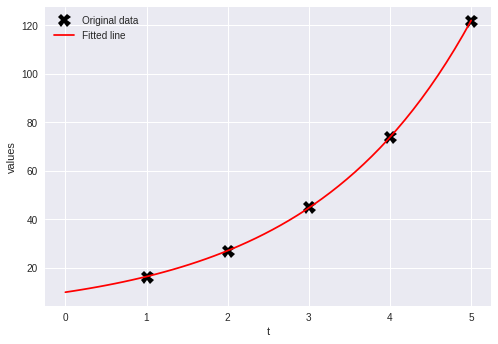
\includegraphics[scale = 0.5]{Boring.png}
\end{center}
\question [10] Consider the time $(T)$ it takes for a runner to complete a marathon ($26$ miles and $385$ yards). Many factors such as height, weight, age, previous training, etc.\ can influence an athlete's performance, but experience has shown that the following three factors are particularly important:
\begin{center}
\begin{tabular}{ll}
$x_1$ = & Ponderal index  = $\frac{\text{height (in.)}}{[\text{weight (lbs.)}]^{1/3}}$, \\
$x_2$ = & Miles run during  the  previous $8$ weeks,\\ 
$x_3$ = & Age (years).
\end{tabular}
\end{center}
A linear model hypothesizes that the time $T$ (in minutes) is given by $T = \alpha_0 +\alpha_1x_1 +\alpha_2x_2 +\alpha_3x_3 +r$, where $r$ is a residual term that accounts for other factors.
\begin{center}
\begin{tabular}{c|ccc}
$T$ & $x_1$ & $x_2$ & $x_3$ \\ \hline
$181$ &  $13.1$ & $619$ & $23$ \\
$193$ & $13.5$ & $803$ & $42$ \\ 
$212$ & $13.8$ & $207$ & $31$ \\ 
$221$ & $13.1$ & $409$ & $38$ \\
$248$ & $12.5$ & $482$ & $45$
\end{tabular}
\end{center}


\begin{parts}
\part Determine the least squares estimates for the coefficients $\alpha_0,\dots,\alpha_3$ from the available data. 

\begin{lstlisting}[language=Python]
def func(a, x1, x2, x3):
  return (a[0] + a[1] * x1 + a[2]*x2 + a[3]*x3)

xdata = np.array([[1,1,1,1,1], [13.1, 13.5, 13.8, 13.1, 12.5],
[619, 803, 207, 409, 482], [23, 42, 31, 38, 45]]).T
ydata = np.array([181, 193, 212, 221, 248])


a = np.linalg.lstsq(xdata, ydata,rcond=None)[0]

# For validation
for i in range (5):
  print(func(a, xdata[i][1], xdata[i][2], xdata[i][3]))  
\end{lstlisting}
$\alpha_0 = 4.92044229e+02$
\\
$\alpha_1 = -2.34354608e+01$
\\
$\alpha_2 = -7.61338932e-02$
\\
$\alpha_3 = 1.86243954e+00$

\part  Estimate the expected marathon time for a 43-year-old runner of height $74$ in., weight $180$ lbs., who has run $450$ miles during the previous eight weeks.
\part Your instructor (height $68$ in., weight $138$ lbs, and $32$ years old) wants to qualify for the Boston Marathon this year.  How many miles should he run in an eight week period before the marathon to qualify for the Boston marathon? (In his age group, the cutoff for qualification is 3 hours 5 minutes). 

\begin{lstlisting}[language = Python]
def func(a, x1, x2, x3):
  return (a[0] + a[1] * x1 + a[2]*x2 + a[3]*x3)

def coeff(a, age, height, weight, mile):
  x1 = height/ weight**(1/3)
  x2 = mile
  x3 = age
  return func(a, x1, x2, x3)
  
# Part b
age = 43
height = 74
weight = 180
mile = 450

ans = coeff(a, age, height, weight, mile)
print(ans)
\end{lstlisting}
Answer = 230.7208607989702
\end{parts}

For part (c), feel free to use a different person (such as yourself, someone you admire, or a famous mathematician) than the instructor. The qualification times are available at this link: \url{https://www.baa.org/2019-boston-marathon-qualifier-acceptances}.
\begin{lstlisting}
def func(a, x1, x2, x3):
  return (a[0] + a[1] * x1 + a[2]*x2 + a[3]*x3)

def coeff(a, age, height, weight, mile):
  x1 = height/ weight**(1/3)
  x2 = mile
  x3 = age
  return func(a, x1, x2, x3)

# Part c
age = 30
height = 76
weight = 160
mile = 200

ans = coeff(a, age, height, weight, mile)
print(ans) 
\end{lstlisting}
Answer = 204.61012886187106
\end{questions}
\end{document}




